\documentclass[twoside, kulak]{kulakreport}
\usepackage[dutch]{babel}
\usepackage{subfiles}
\usepackage{url}
\usepackage{amsmath}
\usepackage{graphicx}
\usepackage{subfig}

\title{Levens redden met machine\\ learning: Support Vector\\ Machines voor tumorclassificatie}
\subtitle{Eindverslag van de teamopdacht}
\author{Team $\exists$uler}
\emailaddress{}
\date{Academiejaar 2023 -- 2024}
\faculty{Groep Wetenschap \& Technologie Kulak}
\group{Bachelor fysica, informatica, wiskunde\\
	ingenieurswetenschappen\\[1ex]
	X0B53A -- Probleemoplossen en ontwerpen, deel 1\\
	X0A22D -- Informaticawerktuigen}
\institute{Vincent Van Schependom, Daan Vanhaverbeke, Jasper Benoit, Lasha Shergelashvili, Marie Taillieu, Zeineb Kharbach, Florian Degraeve, \\Younes Mebarki}
\address{
	\textbf{KU Leuven Kulak} \\
	\textbf{Groep Wetenschap \& Technologie} \\
	Etienne Sabbelaan 53\\
	8500 Kortrijk}

\newcommand{\norm}[1]{\left\| #1 \right\|}

\begin{document}
	
	\titlepage
	
	\tableofcontents
	
	\chapter*{Inleiding}
	
	Dit is het eindverslag van de teamopdracht, waar we met alle leden van team \(\exists\)uler gedurende negen weken aan gewerkt hebben. We maakten doorheen de sessies kennis met machine learning en verwierven week na week meer kennis over dit onderwerp. We oefenden eerst op het onder de knie krijgen van twee basistechnieken, waarna we in week zes begonnen met het uitwerken van onze eigen machine learning toepassing.
	
	\section*{Inhoud van dit eindverslag}
	
	We zullen in dit eindverslag de lezer eerst laten ontdekken wat machine learning precies is. Vervolgens bespreken we wat \textit{supervised learning} inhoudt, in vergelijking met \textit{unsupervised learning}. We bespreken ook wat classificatie juist is. Hierna zal het principe achter Support Vector Machines, de toepassing waarvoor we kozen, volledig uitgelegd worden. Hierbij zullen ook de nodige termen zoals \textit{bias}, variantie en \textit{cross-validation} aan bod komen. Daarna zullen we verschillende classificatietechnieken vergelijken en beargumenteren waarom voor de tumor-dataset SVM een geschikte keuze blijkt te zijn. Tot slot evalueren we de resultaten van SVM op onze dataset.
	
	\section*{De gegevens}
	
	We maken in ons verslag gebruik van de resultaten van een onderzoek naar de verschillende eigenschappen van tumoren bij borstkankerpatiënten. Hierbij onderzochten wetenschappers W. Nick Street, W. H. Wolberg, en O. L. Mangasarian \cite{tumoronderzoek} in 1993 welke kenmerken de meeste invloed hadden in het al dan niet kwaadaardig zijn van een tumor. Deze kenmerken werden berekend op basis van een gedigitaliseerd beeld van een fijne naaldaspiraat (FNA) van de borstmassa. Dergelijke beelden zijn te zien in figuur \ref{fig:borstscan}. De data die in het onderzoek vergaard werd, werd nadien publiekelijk vrijgegeven \cite{tumordataset}, wat ons in de mogelijkheid stelt om de data te verwerken met hedendaagse machine learning technologie.
	
	\begin{figure}
		\hfill
		\subfloat{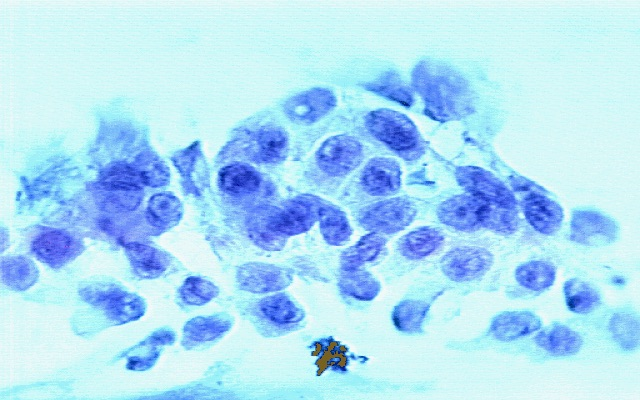
\includegraphics[width=4.5cm]{borstscan2}}
		\hfill
		\subfloat{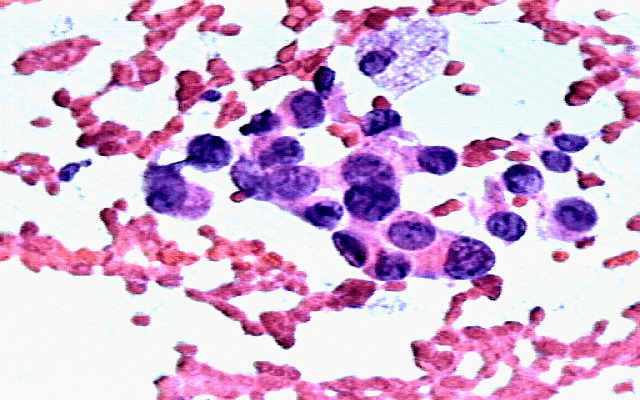
\includegraphics[width=4.5cm]{borstscan}}
		\hfill
		\subfloat{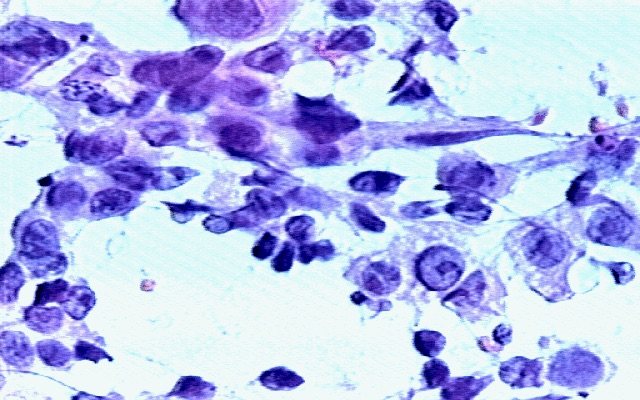
\includegraphics[width=4.5cm]{borstscan3}}
		\hfill
		\caption{Gedigitaliseerde beelden van fijne naaldaspiraten van de borstmassa. \cite{tumoronderzoek}}
		\label{fig:borstscan}
	\end{figure}
	
	\chapter{Situering van SVM binnen machine learning}
	
	\section{Wat is machine learning?}
	
	Machine learning is een tak binnen het gebied van de artificiële intelligentie, waarbij we een model trainen op basis van een gegeven dataset. Naarmate de training vordert, zal het model bepaalde verbanden beginnen leggen en bepaalde structuren beginnen herkennen in de data waarop het getraind wordt. In principe neemt de kwaliteit van het model toe wanneer de data, waarop het model zich baseert, toeneemt.
	
	In dit verslag zal een model getraind worden dat verbanden zal zoeken in de dataset met tumoren van borstkankerpatiënten. Het model zal trachten een link te vinden tussen de verschillende kenmerken van deze tumoren en de klasse waartoe deze tumoren behoren; die van de goedaardige tumoren of die van de kwaadaardige.
	
	\section{Terminologie en notatie}
	
	De dataset beschikt over \(n\) verschillende datapunten. Deze individuele datapunten \(x_i\) hebben elk een eindig aantal kenmerken, die we \textit{features}, \textit{inputs} of \textit{onafhankelijke variabelen} zullen noemen. We duiden de hoeveelheid \textit{features} aan met \(p\). Elk individueel datapunt \(x_i\) uit onze set van datapunten \(x_1,x_2,...,x_n\) is dus van de vorm \(x_i(x_1,x_2,...,x_p)\) (met \( 1 \leq i \leq n \)). Deze features van de dataset kunnen we voorstellen aan de hand van de matrix \(X\), die als volgt gedefinieerd wordt: \[X = \left[ 
	\begin{array}{c}
		x_1 \\
		x_2 \\
		x_3 \\
		\vdots \\
		x_p
	\end{array} \right] = \left[ 
	\begin{array}{ccccc}
		x_{11} & x_{12} & x_{13} & \ldots & x_{1p}  \\
		x_{21} & x_{22} & x_{23} & \ldots & x_{2p} \\
		x_{31} & x_{32} & x_{33} & \ldots & x_{3p} \\
		\vdots & \vdots & \vdots & \ddots & \vdots \\
		x_{n1} & x_{n2} & x_{n3} & \ldots & x_{np}
	\end{array}\right]\]
	
	Hierbij is \(X_{ij}\) de meetwaarde van de \(j\)-e feature voor het \(i\)-e datapunt met met \(i=1,2,3,...,n\) en \(j=1,2,3,...,p\). De tumordataset bevat gegevens over \(569\) tumoren, die elk \(30\) kenmerken hebben. In de dataset \(n\) dus gelijk aan \(569\) en \(p\) gelijk aan \(30\).
	
	\section{Supervised learning}
	
	Machine learning kan worden opgesplitst in twee grote categorieën; \textit{supervised learning} enerzijds en \textit{unsupervised learning} anderzijds. De naam van beide vormen geeft eigenlijk al weg wat deze vormen precies inhouden.
	
	Bij \textit{unsupervised learning} is er voor elk datapunt in de dataset zowel features als outputs voor handen. Er is sprake van zogenaamde 'input-outputparen'. We kunnen ons model trainen op het vinden van een verband tussen de \(x\)-waarden en de \(y\)-waarden in onze trainingsdataset. Het uiteindelijke doel is dan dat het model voor een nieuwe dataset, op basis van de \textit{features} in die dataset, een output zal voorspellen.
	
	Bij \textit{unsupervised learning} zal de data enkel uit inputs of \(x\)-waarden bestaan en zijn er dus geen afhankelijke variabelen. Een \textit{unsupervised learning}-model zal zelf patronen of structuren trachten te vinden in de data en vervolgens de data zelf onderverdelen in klassen. De details achter \emph{unsupervised learning} liggen buiten de scope van dit rapport en zullen we dus achterwege laten.
	
	\subsection{Uitbreiding van de notatie}

	Aangezien we aan \textit{supervised learning} doen, hebben we voor elke input \(x_i\) in de dataset ook een bijhorende \textit{output} \(y_i\). Er zijn dus \(n\) \(y\)-waarden \(y_1,y_2,...,y_n\), die - net zoals de \textit{features} - matricieel kunnen worden voorgesteld als volgt: \[Y =  \left[ \begin{array}{ccccc} y_1 & y_2 & y_3 & \ldots & y_n \end{array} \right]\]
	
	\section{Classificatie}
	
	Classificatie in machine learning is een vorm van supervised learning waarbij het doel is om een input toe te wijzen aan een van de vooraf gedefinieerde klassen. De klassen worden vaak ook aangeduid als \textit{label} of \textit{categorie}. Het ultieme doel van classificatie is om te bepalen in welke categorie nieuwe gegevens zullen vallen.
	
	We passen dit even toe op onze tumordataset. We willen aan de hand van classificatie onderzoeken wat de aard van een tumor is. Er zijn dus twee mogelijke categorieën waartoe een tumor behoort: die van de goedaardige tumoren of die van de kwaadaardige. Elke individuele output \(y_i\) is dus ofwel gelijk aan \(1\) (goedaardig), ofwel gelijk aan \(-1\) (kwaadaardig). Omdat er slechts twee mogelijke klassen zijn, is er sprake van \textit{binaire classificatie}. Er bestaan echter ook classificatietechnieken waar meerdere klassen aan bod komen.
	
	\chapter{Het \textit{maximum margin}-principe}
	
	Het SVM model zal trachten onze datapunten te scheiden in twee klassen. In onze dataset heeft elk datapunt waarde \(-1\) of \(1\), afhankelijk van de klasse waartoe het punt behoort. Indien elk punt in de dataset \(p\) verschillende \textit{features} heeft, zullen er \((p-1)\)-dimensionele objecten, genaamd hypervlakken (of \textit{hyperplanes}), berekend worden om de dataset in deze twee te groepen verdelen. 
	
	We construeren twee zo'n hypervlakken die de twee gegevensklassen scheiden, zodat de afstand daartussen zo groot mogelijk is. Het gebied dat wordt begrensd door deze twee hypervlakken wordt de marge genoemd. Deze marge zal zo groot mogelijk gemaakt worden door het model. Het hypervlak tussen de marge noemen we de beslissingsgrens.
	In het geval dat elk datapunt drie \textit{features} heeft, zal zo'n hypervlak een 2-dimensionaal vlak zijn. In ons geval heeft elk datapunt echter twee \textit{features}, dus kan de dataset gescheiden worden door een rechte, dat strikt genomen een 1-dimensioneel hypervlak is.
	
	\section{De hypervlakken}
	
	We stellen een voorschrift op voor de twee scheidingsrechten, die te zien zijn in figuur \ref{fig:svm}, waartussen zich een marge bevindt. Als \(\vec{w}\) de normaalvector is op de hypervlakken, kunnen we de vergelijkingen van deze rechten schrijven als \(\vec{w}\cdot \vec{x}-b=1\) en \(\vec{w}\cdot \vec{x}-b=-1\). Hierbij is \(b\) dan de \textit{intercept} van de rechte die de beslissingsgrens beschrijft. De \textit{intercept} is de \(y\)-waarde voor \(x=0\). Alle punten boven het eerste hypervlak worden geclassificeerd als horend tot de ene klasse. De punten onder het tweede hypervlak worden geclassificeerd als horende tot de andere klasse.
	
	\begin{figure}[h!]
		\centering
		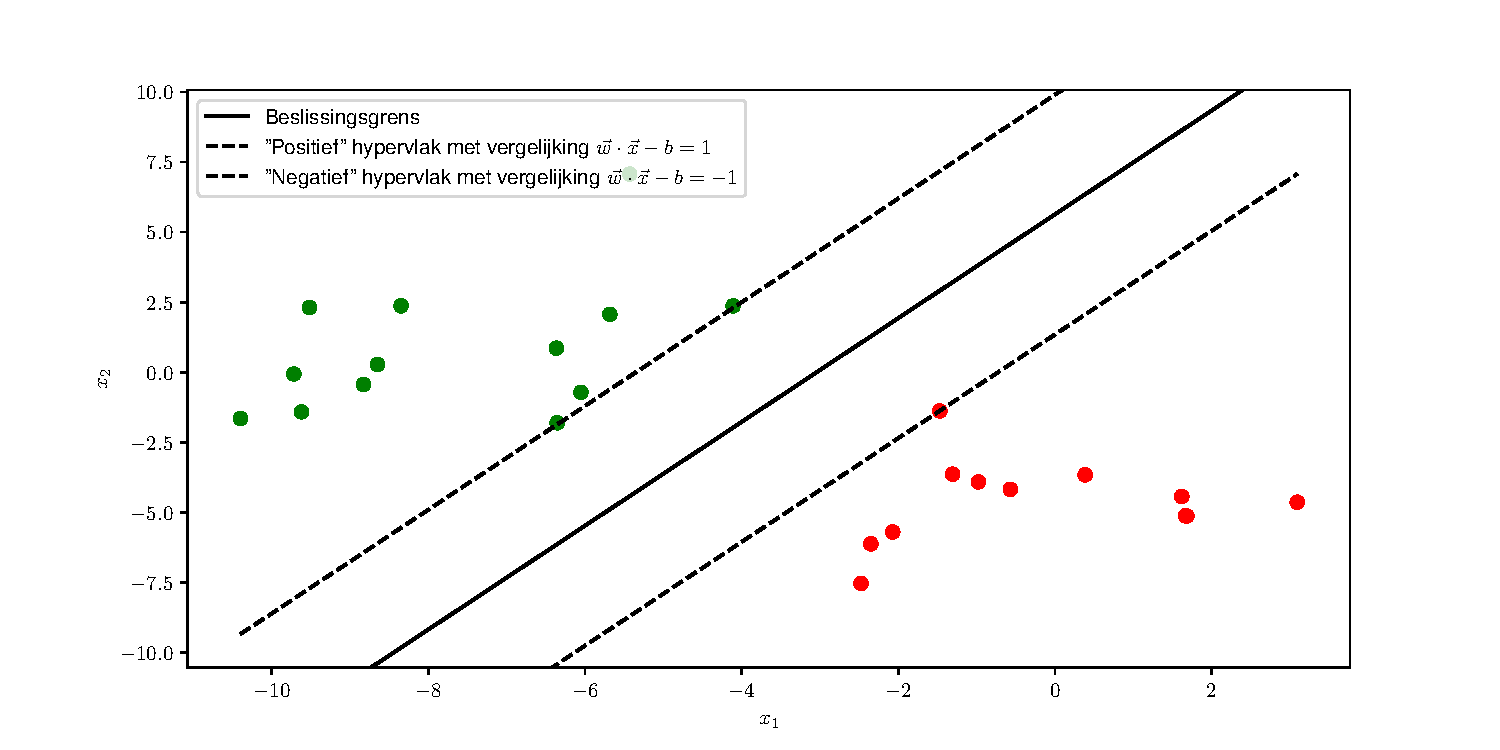
\includegraphics[width=.7\textwidth]{svm-afbeelding}
		\caption{Twee lineair scheidbare wolken van punten. De kleuren van de punten duiden aan tot welke klasse ze behoren.}
		\label{fig:svm}
	\end{figure}
	
	De marge is het gebied tussen deze twee hypervlakken. De breedte van hiervan is gelijk aan \(\frac{2}{\norm{\vec{w}}}\) en aangezien we die breedte willen maximaliseren, zullen we met andere woorden dus \(\norm{\vec{w}}\) trachten te minimaliseren.
	
	\section{De marge maximaliseren}
	
	Als de dataset twee lineair scheidbare 'wolken' vormt en er geen \textit{outliers} - punten die niet tot de juiste wolk behoren - zijn, is het bepalen van de maximale marge vrij makkelijk. Het wordt moeilijker wanneer er wel \textit{outliers} zijn en de twee wolken dus niet meer perfect lineair scheidbaar zijn, zonder dat punten aan de verkeerde kant van de twee hyperplanes belanden. Daarom voeren we een soort foutterm in. 
	
	\subsection{\textit{Hinge loss}}
	
	De \textit{hinge loss} is een soort foutterm die we toevoegen aan punten die niet goed of met geen grote zekerheid worden geclassificeerd. Deze \textit{hinge loss} wordt berekend door de formule \[\max{(0,1-y_i(\vec{w}\cdot\vec{x}_i-b))}\] Deze foutterm laat ons toe om de fouten te beperken, terwijl we de marge maximaliseren. Voor elk punt hebben we dan twee mogelijkheden wat de waarde van de \textit{hinge loss} betreft:
	
	\begin{enumerate}
		\item Het punt met afhankelijke variabele \(y_i\) werd correct geclassificeerd.
		
		Dan ligt het punt dus aan de juiste kant van een van de twee hyperplanes. In dit geval is \(y_i(\vec{w}\cdot\vec{x}_i-b)\ge1\) en zal \(1 - y_i(\vec{w}\cdot\vec{x}_i-b)\le0\). Omdat de \textit{hinge loss} het maximum neemt van 0 en dit laatste getal - dat ofwel ook 0, ofwel negatief is - zal de \textit{hinge loss} in dit geval 0 zijn.
		
		\item Het punt ligt in de marge of het punt ligt aan de verkeerde kant van de beslissingslijn. 
		
		De \textit{hinge loss} wordt dan \(1 - y_i(\vec{w}\cdot\vec{x}_i - b)\). Indien het datapunt binnen de marge ligt, zal de hinge loss tussen 0 en 1 liggen. Het punt wordt dan met lagere zekerheid geclassificeerd, maar we willen het ook niet te hard bestraffen. Indien een datapunt buiten de marge, maar aan de verkeerde kant van de beslissingslijn ligt, zal de \textit{hinge loss} groter dan 1 zijn. We willen het model wel hard bestraffen, want zo'n fouten willen we miniem houden.
	\end{enumerate}
	
	\subsection{De kostfunctie}
	
	Om het SVM-model te trainen, moeten we nu dus met twee zaken rekening houden. Enerzijds willen we \(\norm{\vec{w}}\) minimaliseren om een zo groot mogelijke marge te bekomen anderzijds willen we de \textit{hinge loss} of strafterm zo klein mogelijk houden. We voeren een kostfunctie \(J\) in en zoeken het minimum \(\min_{w, b}J\) van deze functie. Het minimalisatieprobleem wordt dan gegeven door de formule \[\min_{w, b}J=\min_{w, b}\left[\frac{1}{n}\sum_{i=1}^n{\max{[0,1-y_i(\vec{w}\cdot\vec{x}_i-b)]}} + \lambda\cdot{||\vec{w}||}^2\right]\]
	
	Hierbij is \(\frac{1}{n}\sum_{i=1}^n{\max{[0,1-y_i(\vec{w}\cdot\vec{x}_i-b)]}}\) de gemiddelde \textit{hinge loss}, dus de gemiddelde foutterm die werd toegekend over alle \(n\) datapunten in de dataset. De tweede term \(\lambda\cdot{||\vec{w}||}^2\) regelt het evenwicht tussen enerzijds het minimaliseren van de fouten op de trainingsdata en anderzijds het maximaliseren van de marge. \(\lambda\) is een metaparameter van het model en deze parameter vertelt aan het model hoeveel belang we hechten aan het minimaliseren van \(\norm{\vec{w}}\).
	
	\chapter{De regularisatieparameter \(\lambda\)} 
	
	\section{Wat is een metaparameter?}
	
	Machine learning modellen hebben over het algemeen een of meerdere \textit{metaparameters} die de flexibiliteit van het model beïnvloeden. Het model zal zich meer of minder aanpassen aan de trainingsdata naar gelang de waarden van deze metaparameter(s). Deze parameter wordt voor SVM ook wel de \textit{regularisatieparameter} genoemd en wordt aangeduid met \(\lambda\). Deze \(\lambda\) zal uiteindelijk de breedte van de marge - en dus de variabiliteit van het model - beïnvloeden (zie later). 
	
	In het geval van SVM noemen we de metaparameter \(\lambda\) ook wel de \textit{regularisatieparameter}. Deze parameter bepaalt de breedte van de marge en dus ook de variabiliteit van het model:
	
	\begin{itemize}
		
		\item Als \(\lambda\) klein - en eventueel zelfs \(0\) - is, komt het berekenen van een minimale kostfunctie $J$ neer op het op nul zetten van zo veel mogelijke \textit{hinge losses} van zo veel mogelijk punten. Dit resulteert in een kleine marge. 
		
		\item Als \(\lambda\) groot is, ligt er meer nadruk op het minimaliseren van de grootte van \(\norm{\vec{w}}\) en dan spelen de \textit{hinge losses} een minder grote rol. Hoe kleiner \(\norm{\vec{w}}\), hoe groter de marge, want de marge is \(\frac{2}{\norm{\vec{w}}}\) breed. We concluderen dat \(\lambda\) resulteert in een grotere marge, zoals te zien is in figuur \ref{fig:lambda}.
		
	\end{itemize}
	
	\begin{figure}
		\centering
		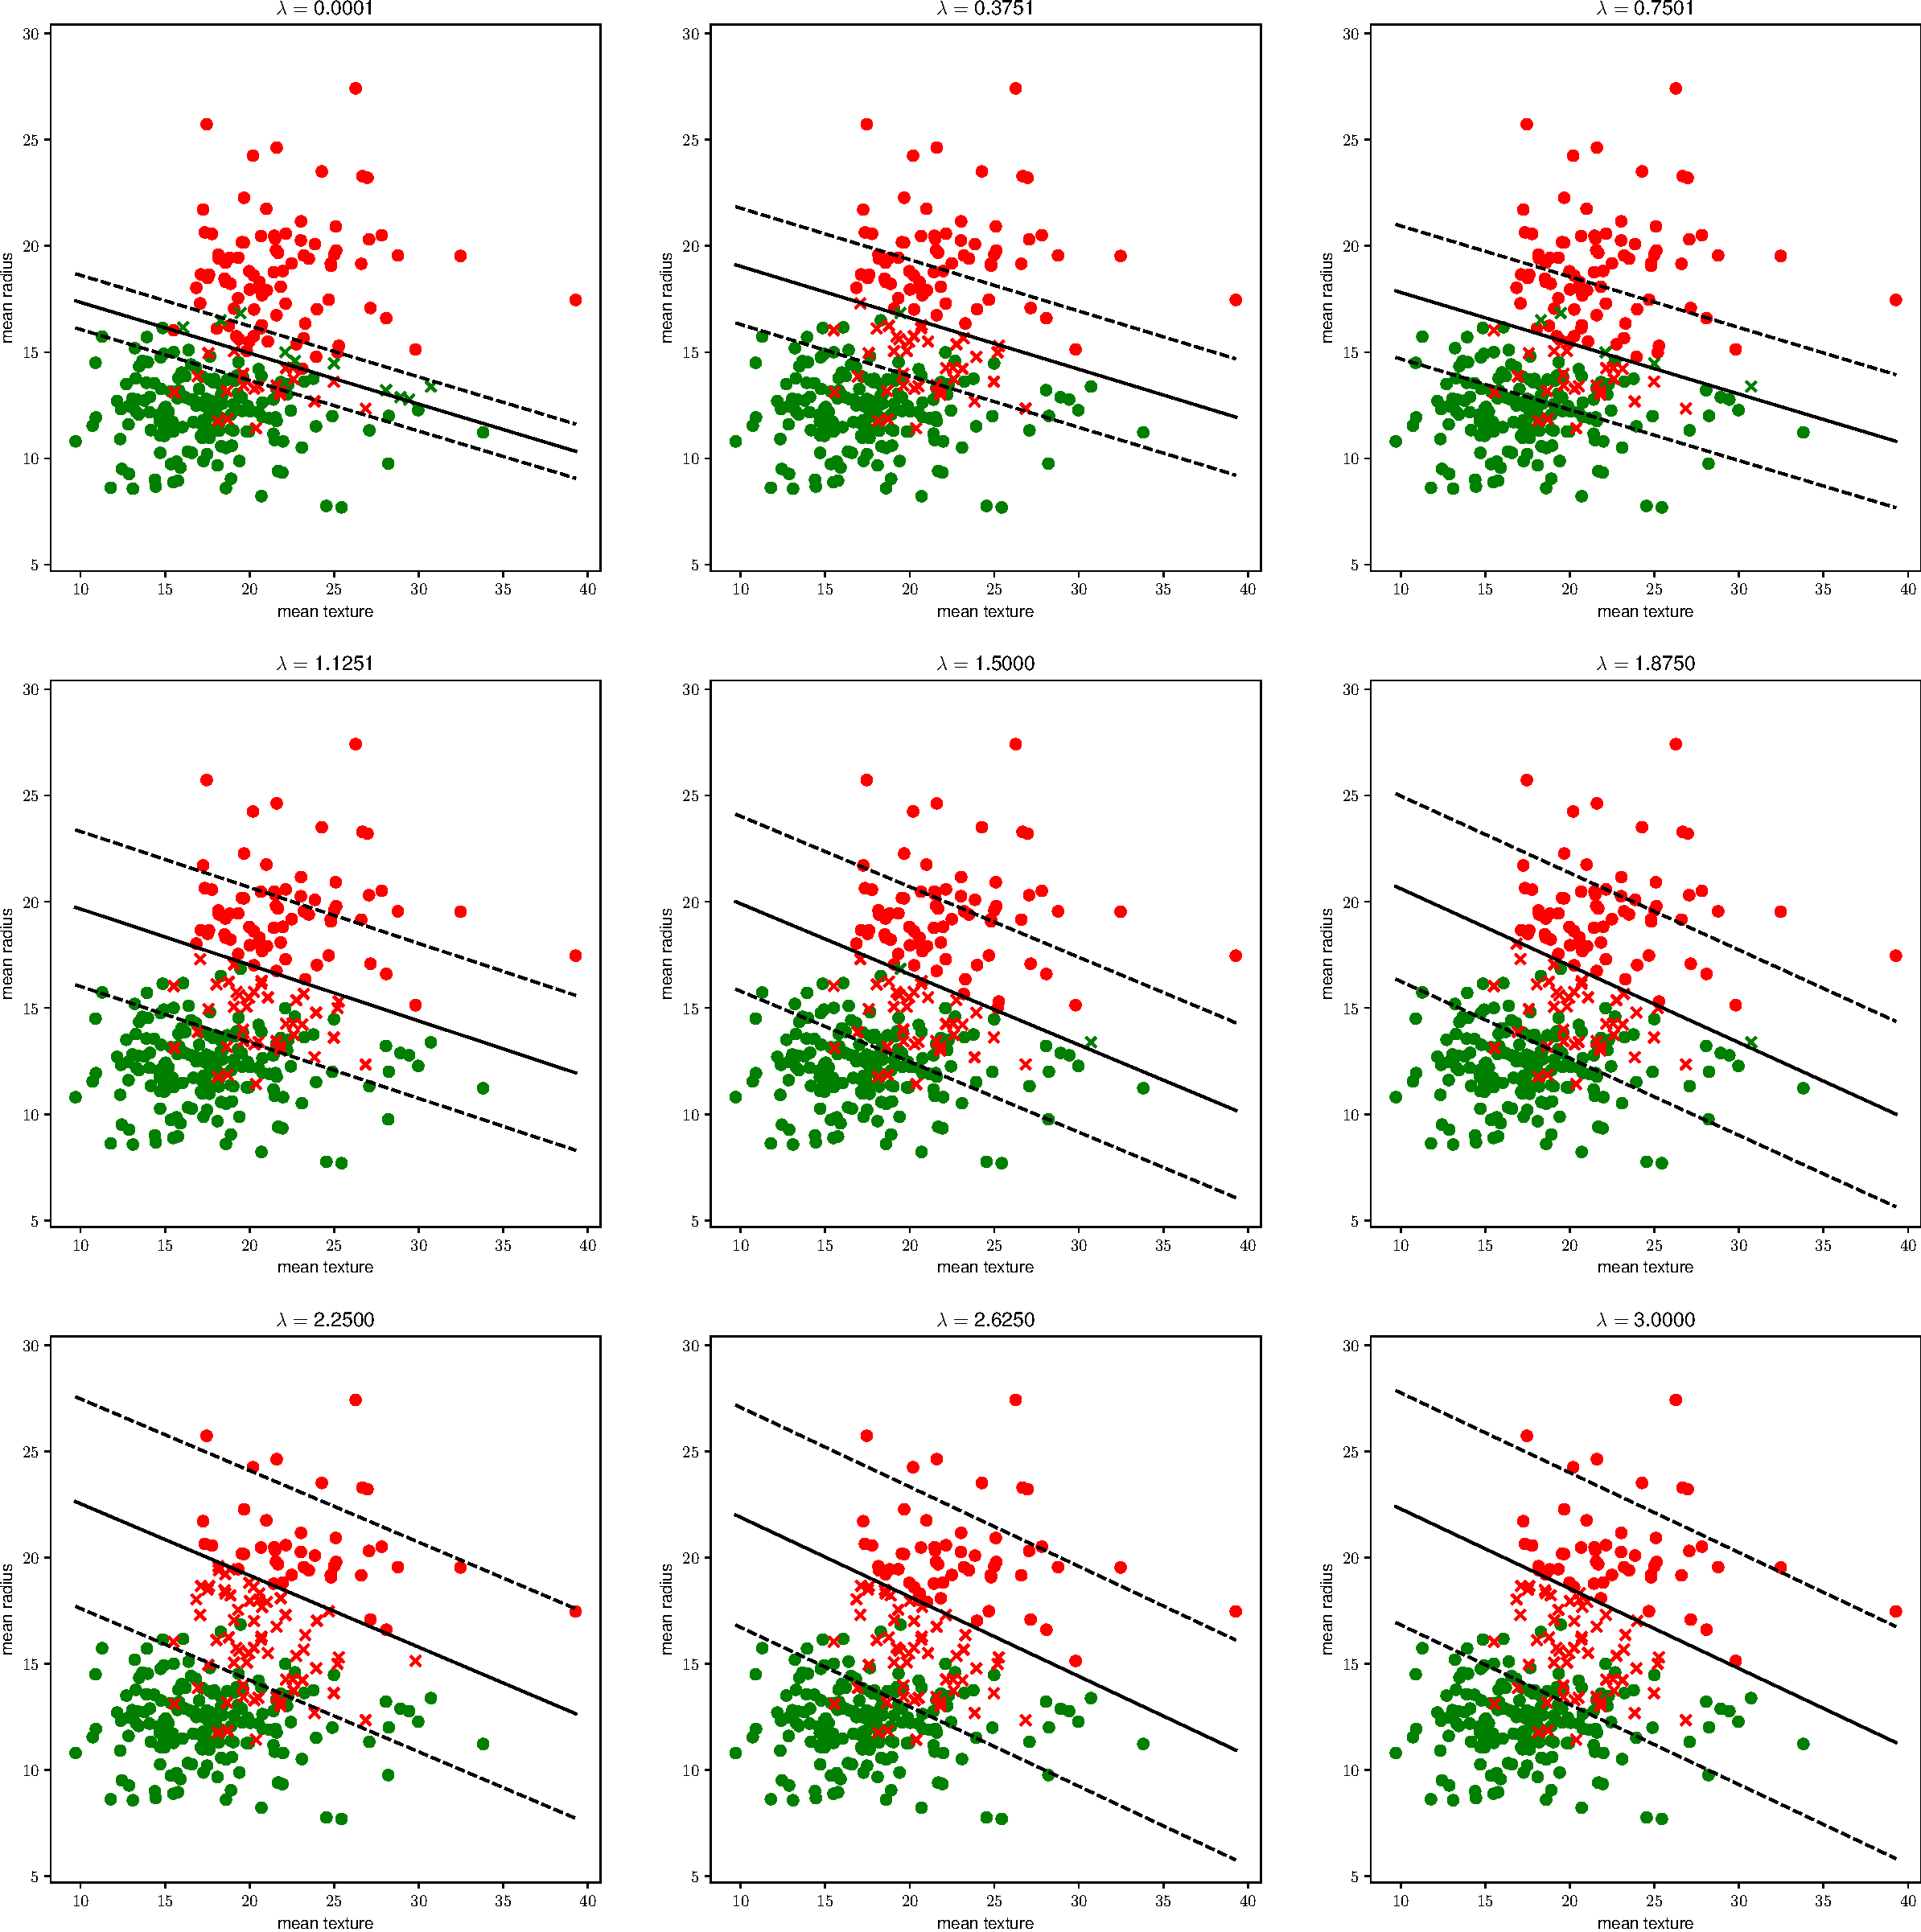
\includegraphics[width=.9\textwidth]{lambda}
		\caption{De invloed van de metaparameter \(\lambda\) op het SVM-model. Een grote \(\lambda\) resulteert in een grote marge, een kleine \(\lambda\) resulteert in een kleine marge.}
		\label{fig:lambda}
	\end{figure}
	
	\section{Het belang van de regularisatieparameter}
	
	Een metaparameter in machine learning - bij ons dus de regularisatieparameter \(\lambda\) - regelt zowel de correctheid als de flexibiliteit van het model. Die twee eigenschappen noemen we respectievelijk \textit{bias} en variantie.
	
	\subsection{Bias}
	
	In machine learning verwijst \textit{bias} naar de systematische fout die door een model wordt geïntroduceerd wanneer het de onderliggende patronen in de trainingsgegevens consequent verkeerd weergeeft. Dit kan leiden tot onnauwkeurige voorspellingen en onbetrouwbare prestaties op nieuwe datasets. 
	
	\newpage
	
	Als een classificatiemodel wordt getraind op vertekende gegevens die overwegend één klasse vertegenwoordigen, kan het model leren nauwkeuriger te zijn voor die groep, terwijl het slecht presteert voor andere groepen. Als we ons SVM model bijvoorbeeld bijna uitsluitend trainen op gevallen waar de tumor kwaadaardig is, zal het hoogstwaarschijnlijk niet goed presteren voor nieuwe datapunten waar de tumor goedaardig is. Het model is namelijk niet getraind op tumoren van die aard en zal dus geen nauwkeurige predicties kunnen doen. De \textit{bias} is in dit geval zeer hoog.
	
	Het kan echter ook gebeuren dat de trainingsgegevens niet representatief zijn voor de populatie waarnaar ze willen generaliseren. Dit probleem treedt op wanneer bepaalde groepen in de populatie onder- of oververtegenwoordigd zijn in het trainingspakket. Als we ons SVM model bijvoorbeeld enkel trainen op tumoren van vrouwelijke borstkankerpatiënten, is de kans dat het model slecht presteert voor een nieuwe dataset van mannelijke patiënten vrij groot. We trainen ons model dan niet per se voornamelijk op één classificatiegroep, zoals in het vorige voorbeeld, maar de trainingsdata is eveneens niet representatief.
	
	\subsection{Variantie}
	
	De variantie is de maat voor de gevoeligheid van het model. Het geeft inzicht over de flexibiliteit van een model, met name hoe nauwkeurig de voorspellingen zijn bij verschillende datasets.
	
	Bij een hoge variantie is het model sterk aangepast aan de trainingsdata. Dit betekent dat zelfs kleine veranderingen in de trainingsdata een grote invloed zullen hebben op het model, wat resulteert in een fenomeen genaamd \textit{overfitting}. In het geval van tumorclassificatie zou een hoge variantie betekenen dat het model zeer nauwkeurig kan voorspellen of een tumor goedaardig is bij de trainingsdata. Maar doordat het model te sterk is afgestemd op de trainingsdata, zal het moeite hebben met generaliseren en levert dit geen precieze voorspellingen op voor de andere datasets, met name de validatie- en testdatasets.
	
	Aan de andere kant kan een model ook een te lage variantie hebben. Dit betekent dat het model te veel generaliseert en weinig verandert indien de trainingsdata verandert. Een te lage variantie leidt tot \textit{underfitting}. Hierdoor levert het ook geen betrouwbare voorspellingen op. Toegepast op tumorclassificatie zal een te lage variantie leiden tot een te sterk gegeneraliseerd model, waarbij het model niet goed presteert op de drie verschillende datasets.
	
	\section{\textit{Bias-variance trade-off}}
	
	We willen enerzijds de \textit{bias} minimaliseren door te fouten die ons model maakt te beperken. Dit kunnen we doen door ons model flexibeler te maken. Een grotere flexibiliteit resulteert onvermijdelijk echter in een grotere variantie. Een grote variantie resulteert dan in \textit{overftting}, wat we natuurlijk ook willen vermijden, aangezien ons model anders geen accurate voorspellingen zal doen op nieuwe data. Het vinden van een evenwicht tussen de \textit{bias} en de variantie is dus cruciaal voor het trainen van ons model. We noemen dit probleem vaak ook de \textit{bias-variance trade-off}. Aangezien zowel de \textit{bias} als de variantie worden beïnvloed door de regularisatieparameter, zullen we de beste waarde voor \(\lambda\) zoeken.
	
	\section{\textit{Cross-validation}}
	
	\subsection{De data opsplitsen}
	
	Voor het vinden van de optimale waarde \(\lambda_{\text{opt}}\) voor de regularisatieparameter, maken we gebruik van een principe genaamd \textit{cross-validation}. Hiervoor splitsen we eerst de data die we voor handen hebben op in 3 delen: 50\% trainingsdata, 25\% validatiedata, 25\% testdata:
	
	\begin{description}
		\item [Trainingsdata]: 285 tumoren
		\item [Validatiedata]: 142 tumoren
		\item [Testdata]: 142 tumoren
	\end{description}
	
	Voor \textit{cross-validation} zullen we enkel gebruik maken van de eerste twee datasets. De testdata komt helemaal op het einde van dit verslag aan bod, wanneer we de accuraatheid van ons model zullen evalueren op nieuwe data.
	
	\subsection{Itereren over verschillende waardes voor \(\lambda\)}
	
	Na deze opsplitsing kunnen we ons model trainen op de validatiedata, telkens met een verschillende waarde voor \(\lambda\). Bij elke iteratie zullen we de accuraatheid van het model voor deze specifieke waarde van de regularisatieparameter evalueren aan de hand van de trainingsdata. We herhalen onderstaand proces voor \(100\) verschillende waarden van \(0.0001\) tot \(8\) voor \(\lambda\):
	
	\begin{itemize}
		\item Train het model op basis van onze trainingsdata voor een bepaalde waarde van \(\lambda\). Deze trainingsdata bestaat uit 285 datapunten (met elk 30 \textit{features}) en 285 \textit{outputs}.
		\item Maak een voorspelling met dit model op basis van de \textit{inputs} van de validatiedataset.
		\item Vergelijk de voorspellingen voor de \(y\)-waarden van de validatiedata met de effectieve \(y\)-waarden van de validatiedataset en bereken op basis daarvan de accuraatheid van het model voor de huidige waarde van \(\lambda\). Hiervoor delen we het aantal goed geclassificeerde punten in de validatiedata door het aantal verkeerdelijk geclassificeerde punten in de validatiedata. Door dit getal te vermenigvuldigen met \(100\), krijgen we een percentage dat dan de accuraatheid van het model beschrijft.
	\end{itemize}
	
	We kunnen de accuraatheid van het getrainde model de trainingsdata uitzetten in functie van een metaparameter met behulp van een grafiek, zoals te zien is in figuur \ref{fig:metaparameter}. We kiezen de \(\lambda\) die ons de hoogste accuraatheid oplevert: \(\lambda_{\text{opt}}=0.727\). Met deze waarde voor de regularisatieparameter was de accuraatheid van het model tegenover de validatiedata meer dan \(85\%\).
	
	\begin{figure}
		\centering
		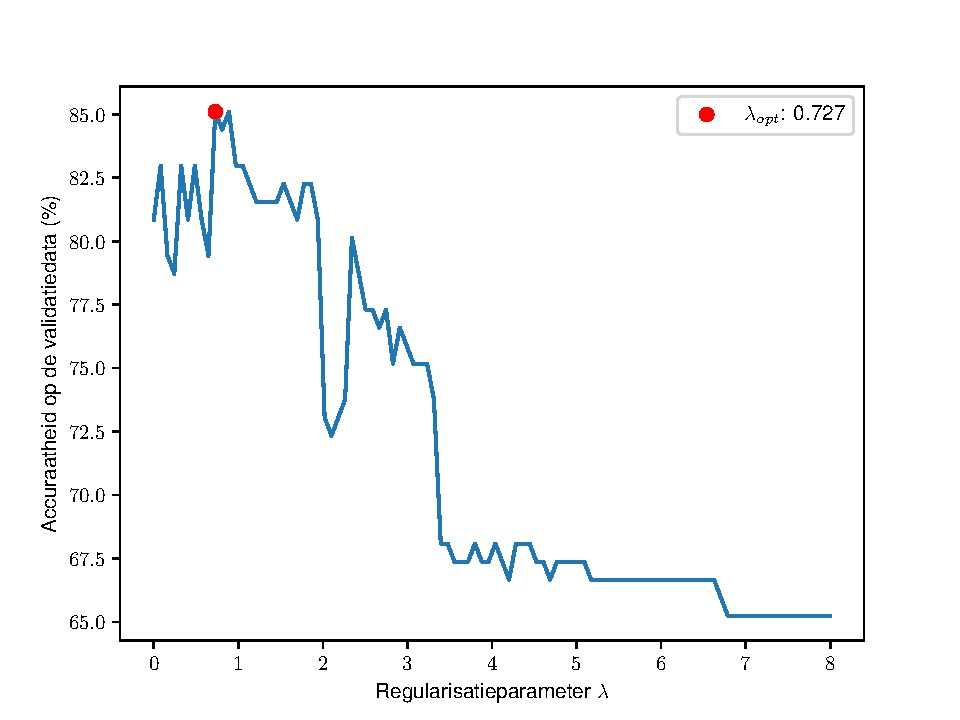
\includegraphics{accuraatheid}
		\caption{De accuraatheid van het model t.o.v. de validatiedata, uitgezet in functie van de metaparameter \(\lambda\) voor ons SVM-model.}
		\label{fig:metaparameter}
	\end{figure}
	
	\chapter{Vergelijking met andere classificatietechnieken}
	
	Waar Support Vector Machines in uitblinken, is het verwerken van datasets waarvan de datapunten elk zeer veel \textit{features} hebben. SVM werkt namelijk uitermate goed in hoger dimensionale ruimtes, die we helaas dus niet visueel kunnen illustreren. Zo zouden we de tumoren met zeer hoge accuraatheid kunnen classificeren indien we de volledige lijst kenmerken in acht nemen.
	
	Daarnaast is SVM minder gevoelig voor \textit{overfitting} in vergelijking met complexere modellen zoals neurale netwerken. Dit is vooral belangrijk wanneer de data die voorhanden is, eerder beperkt is in grootte. SVM zal dus voor kleinere datasets heel goed presteren, met name als het aantal \textit{features} groter is dan het aantal datapunten. Ook zal SVM in vergelijking met neurale netwerken bij het toevoegen van extra punten minder snel de mist in gaan zoals op figuur \ref{fig:NeuralNetsVsSVM}. Dit is waarom de hyperplane zo belangrijk is bij SVM. 
	
	Indien er heel veel variabiliteit is in de dataset, zal SVM ook een voordeel hebben tegenover andere classificatietechnieken: juist door het feit dat de marge tussen de scheidingshypervlakken zo groot mogelijk wordt gehouden, zullen \textit{outliers} of andere vormen van ruis in de dataset niet in acht worden genomen. SVM is dus totaal niet gevoelig voor \textit{overfitting}. Dit wordt nog eens extra benadrukt aan de hand van figuur \ref{fig:LogistischeRegressieVsSVM}.
	
		\begin{figure}
		\centering
		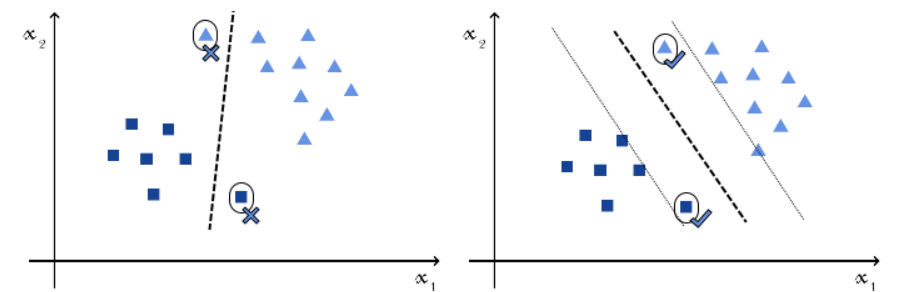
\includegraphics[width=.7\textwidth]{NeuralNets-vs-SVM}
		\caption{Deze figuur uit bron \cite{Luca_2022} geeft een belangrijk verschil tussen een neuraal netwerk en een SVM model weer. Links wordt de werking van een neuraal netwerk geïllustreerd, rechts die van een SVM model. Hierbij valt op dat de kans dat een nieuw datapunt juist geclassificeerd zal worden, veel groter is bij SVM. Deze figuur benadrukt dus ook belang van het \textit{maximum margin} hypervlak bij het voorkomen van \textit{overfitting}. }
		\label{fig:NeuralNetsVsSVM}
	\end{figure}
	
	\newpage
	
	\begin{figure}
		\centering
		\subfloat{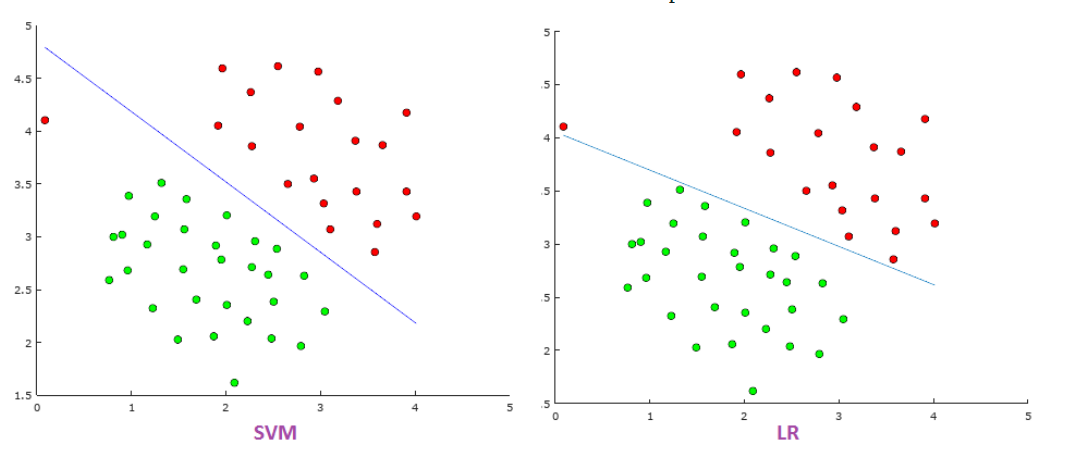
\includegraphics[width=0.9\textwidth]{LogistischeRegressie-vs-SVM}}
		\caption{Deze figuur uit bron \cite{Ramo_2017} toont de vergelijking tussen SVM en logistische regressie. Hierbij valt het duidelijk op dat wanneer er sprake is van een \textit{outlier}, logistische regressie zich heel hard aanpast aan deze \textit{outlier}. Dit toont dan aan dat Support Vector Machines veel beter bestendig zijn tegen ruis in de dataset. }
		\label{fig:LogistischeRegressieVsSVM}
	\end{figure}
	
	Wanneer SVM bij de classificatie van punten van twee \textit{features} geplot wordt, is deze visuele voorstelling ook eenvoudig te begrijpen. Het is namelijk zeer duidelijk of een punt nu tot de ene of andere klasse behoort volgens het model, door naar de eenvoudige scheidingslijn te kijken. Deze interpretatie is moeilijker bij andere classificatietechnieken zoals KNN-classificatie. Deze classificatietechniek berekent een scheidingslijn door naar de K dichtstbijzijnde buren van elk datapunt te kijken, wat vaak resulteert in een ietwat chaotische en minder makkelijk te begrijpen figuur, zoals je kan zien in figuur \ref{fig:KNNvsSVM}. 
	
	\begin{figure}
		\centering
		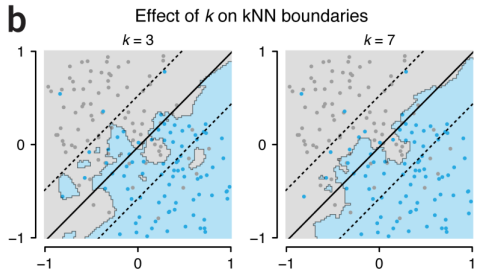
\includegraphics[width=.6\textwidth]{KNN-vs-SVM.PNG}
		\caption{Deze figuur uit bron \cite{bzdok2018machine} vergelijkt KNN-classificatie met SVM-classificatie. Bij de eerste van de twee technieken ontstaan er twee twee gebieden, die worden bepaald door naar de \(k\) dichtste buren te kijken van elk datapunt. Op de linkerfiguur is \(k=3\), op de rechterfiguur is \(k=7\). Met behulp van \textit{cross-validation} werd bepaald dat \(k=7\) de optimale waarde is voor de metaparameter \(k\), met een accuraatheid van 87\%. De rechte die door de grafiek gaat, is de beslissingsgrens van SVM en de stippellijnen zijn hypervlakken. Hierbij valt het duidelijk op dat SVM veel makkelijker te interpreteren is in vergelijking met KNN, terwijl de accuraatheid van SVM nog steeds gelijk is aan 85\% in dit voorbeeld. We boeten, door gebruik te maken van SVM, dus een slechts een klein beetje in op accuraatheid, maar dit is in het voordeel van de interpreteerbaarheid van het model.}
		\label{fig:KNNvsSVM}
	\end{figure}
	
	Tot slot is SVM zeer geheugenefficiënt: het model houdt enkel rekening met de dichtste punten tot de hypervlakken en zal dus, in tegenstelling tot bijvoorbeeld logistische regressie, niet met elk punt rekening moeten houden in de berekening van de beste beslissingsgrens.
	
	\chapter{Resultaten op onze dataset}
	
	\section{\textit{Features}}
	
	Zoals in de inleiding reeds vermeld werd, bestaat onze dataset uit een \(500\)-tal datapunten met elk \(30\) \textit{features}. Hieronder lijsten we de eerste \textit{features} op om de lezer een idee te geven van de data die voor handen is:
	
	\begin{itemize}
		\item Straal
		\item Textuur (standaardafwijking van grijswaarden)
		\item Omtrek
		\item Oppervlakte
		\item Gladheid (lokale variatie in straallengtes)
		\item Compactheid (\(omtrek^2 / oppervlakte - 1.0\))
		\item Concaafheid (ernst van concave delen van de contour)
		\item Concave punten (aantal concave delen van de contour)
		\item Symmetrie
		\item ...
	\end{itemize}
	
	\subsection{Limitaties}
	
	Zoals eerder reeds vermeld werd, botsen we tegen een limitatie wat betreft het aantal \textit{features} die we kunnen gebruiken voor ons model. Indien we het aantal \textit{features} opdrijven, worden de wiskundige berekeningen namelijk een pak complexer. Daarnaast wordt het visueel voorstellen van de dataset ook des te moeilijker bij een toenemend aantal \textit{features}. Wegens deze twee limitaties, zullen we ons dus beperken tot slechts twee \textit{features} per tumor.
	
	\subsection{Selectie}
	
	Hoe selecteren we nu de meest interessante \textit{features}? We kunnen daarvoor gebruik maken van een \textit{pairplot}, zoals er een te zien is in figuur \ref{fig:pairplot}. Een \textit{pairplot} is een visuele weergave van de relatie tussen paren van \textit{features} in een dataset. In machine learning worden dit soort voorstellingen vaak gebruikt om patronen en verbanden tussen de verschillende \textit{features} van een dataset te identificeren. Op basis van deze pairplot bepaalden wij dat \textit{mean texture} (textuur) en \textit{mean radius} (straal) twee interessante \textit{features} waren om te bestuderen.
	
	\begin{figure}
		\centering
		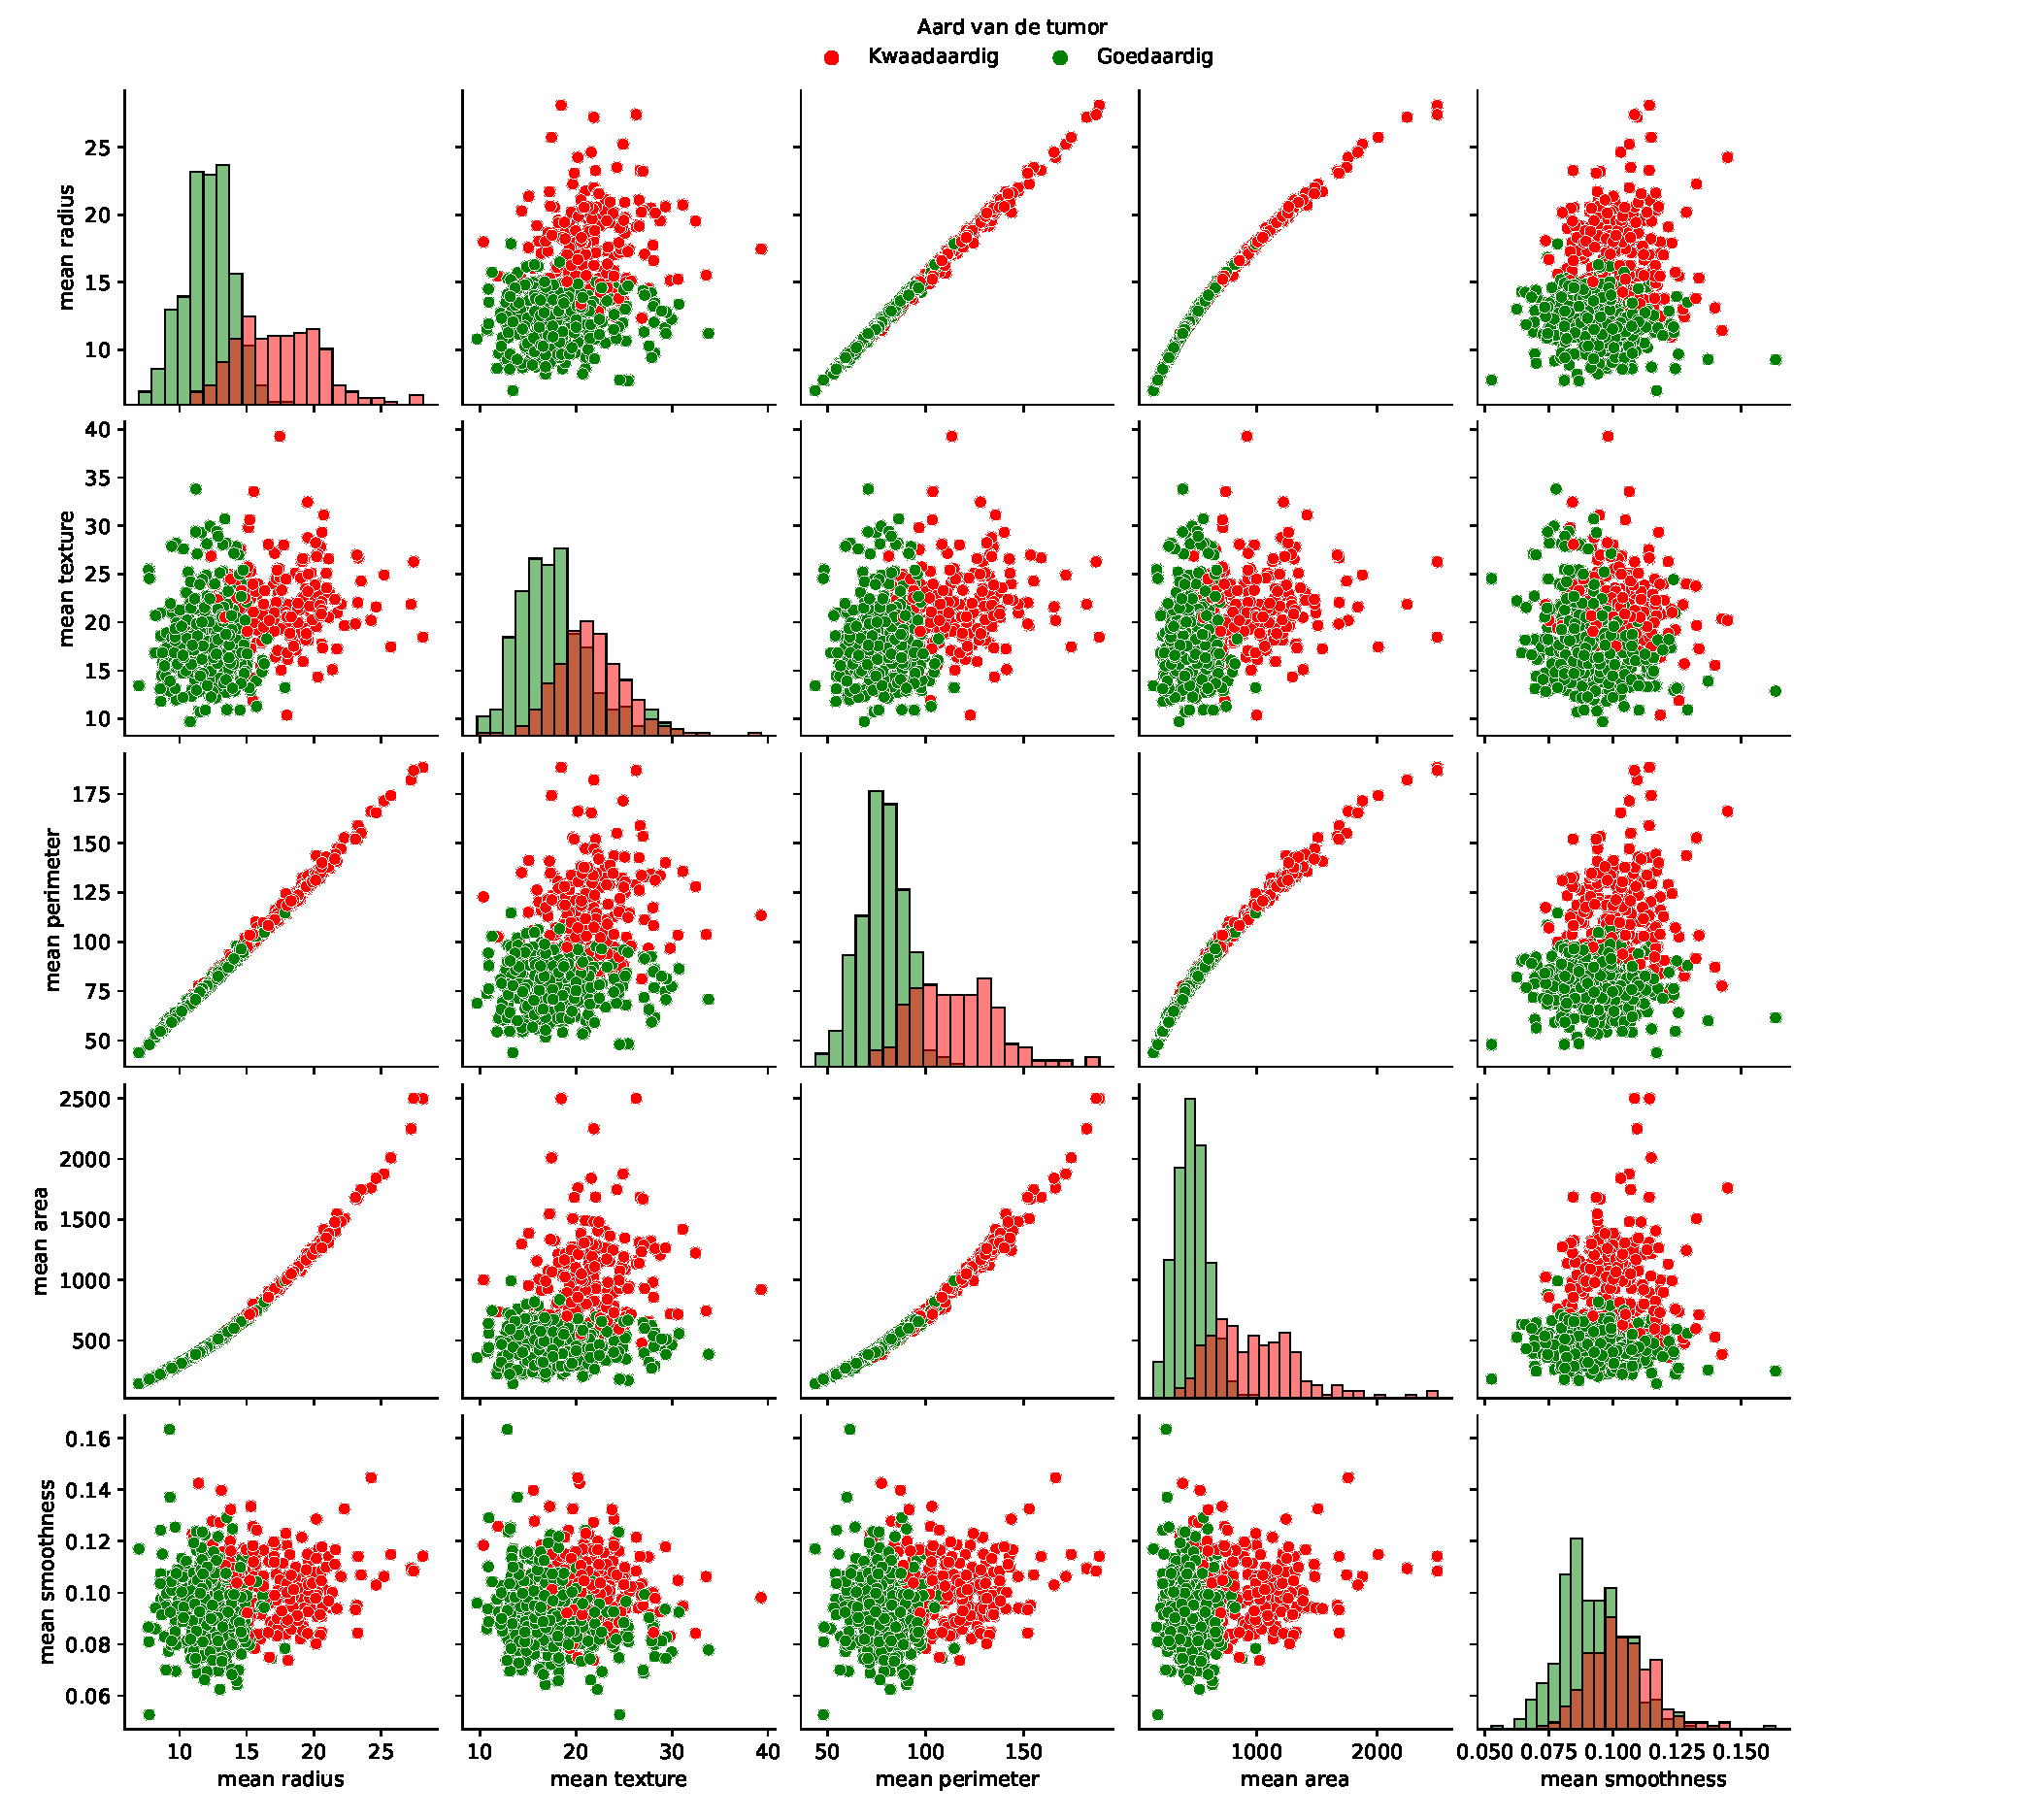
\includegraphics[width=1\textwidth]{pairplot}
		\caption{Een \textit{pairplot} van de eerste 5 \textit{features} in de tumordataset.}
		\label{fig:pairplot}
	\end{figure}
	
	\section{Evaluatie van de accuraatheid}
	
	We trainden ons model op onze trainingsdata, beperkt tot de twee \textit{features} die we hierboven kozen. Via \textit{cross-validation} bepaalden we de optimale waarde voor de regularisatieparameter \(\lambda\). De laatste stap in het proces is om met ons model een voorspelling te maken voor de testdata. Op die manier krijgen we een goed beeld van de effectieve accuraatheid van het model indien het data te zien krijgt waarop het niet getraind is. Zoals te zien is in figuur \ref{fig:testdata}, was ons model in staat om voorspellingen te doen met een accuraatheid van maar liefst \(89,51\%\) op onze testdata.
	
	\begin{figure}
		\centering
		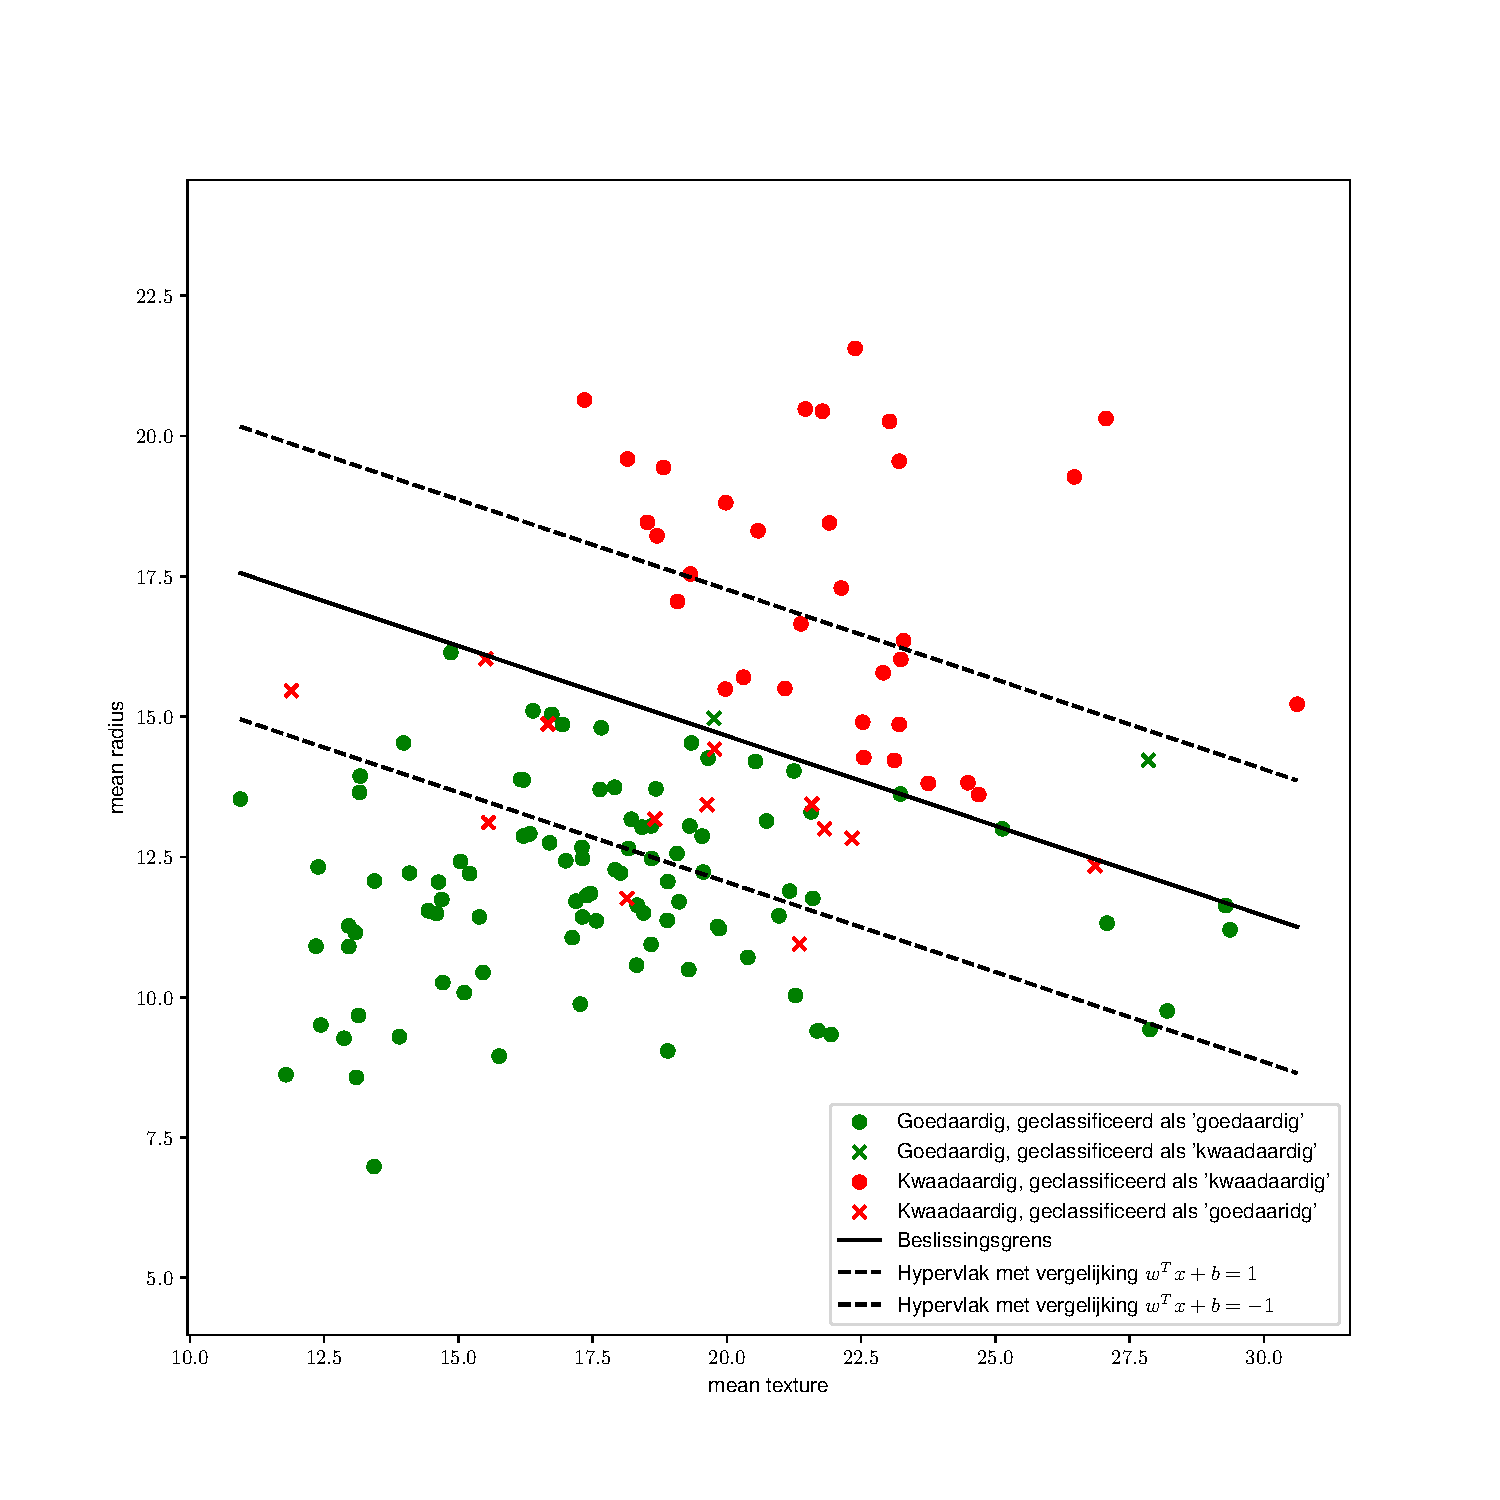
\includegraphics[width=.9\textwidth]{testdata}
		\caption{Ons SVM model toegepast op de testdata. We konden een accuraatheid van \(89,51\%\) bewerkstelligen.}
		\label{fig:testdata}
	\end{figure}
	
	\chapter*{Besluit}
	
	Uit ons onderzoek kunnen we concluderen dat Support Vector Machines een classificatietechniek is die heel wat voordelen heeft dankzij de unieke eigenschappen van het model. De punten worden namelijk gescheiden met behulp van \textit{maximum margin} hypervlakken. Dit wil zeggen dat de marge tussen de hypervlakken zo groot mogelijk gemaakt wordt, wat belangrijk is voor het minimaliseren van foute voorspellingen. Daarnaast viel het ons op dat wanneer er een \textit{outlier} aan onze data wordt toegevoegd, er weinig invloed is op het definitieve model. SVM is dus zeer bestendig tegen \textit{overfitting} en kan daarom ook  gebruikt worden voor kleinere datasets.
	
	Tijdens het trainen van het model wordt de \textit{hinge loss} berekend als foutterm, waarbij de focus ligt op het minimaliseren hiervan. Zo wordt een nauwkeurige classificatie van punten buiten de hypervlakken verzekerd. Omdat we deze fout willen minimaliseren, maar toch een bruikbaar model willen overhouden, ontstaat er de kostfunctie \(J\). Deze functie maakt een balans tussen de foutterm en de breedte van marge tussen de hypervlakken. Hierbij wordt een regularisatieparameter ingevoerd. Deze wordt vervolgens geoptimaliseerd om een zo hoog mogelijke accuraatheid te verkrijgen en toch nog een leesbaar model over te houden.
	
	Na ons model in het algemeen berekend te hebben, pasten we deze toe op een concrete dataset. Met deze dataset wilden we bepalen op basis van enkele \textit{features} of een tumor goedaardig of kwaadaardig is. Uit deze \textit{features} kozen we er twee die werden toegepast op ons SVM-model. Hierbij verkregen we een accuraatheid van \(89,52\%\), waaruit we konden besluiten dat SVM de beste manier is om een tumor te classificeren als goedaardig of kwaadaardig.
	
	\nocite{enwiki:1183475870}
	\nocite{mediumarticle}
	\nocite{bzdok2018machine}
	
	\bibliographystyle{unsrt}
	\bibliography{referenties}
	
\end{document}
